\adparagraph{Spearman Distance}
In Figure \ref{fig:footruledistance} are the results of the SFD tests. As in KTD it is normalized to be between 0 and 1 where if 0 the list are equal.

In general the tendencies are very similar to those of KTD and the approaches follow the same curve with all most the same distance jumps between the group sizes. This can be noted in Table \ref{tbl:sfd}.

Not surprisingly SF performs the best in this test. This is due to it have a natural advantage when using SFD as they are based on the same principle. This somewhat deems its result in this test invalid.

Avg again performs the worst when looking at the SFD results. This is for the same reason as with the SFD measure, Avg does not take the rank of items into account.

For \MC and BC we get some interesting results. They still follow each other really close. However in this test \MC perform marginally better in the most cases except at group size 12 and 16 where BC is slightly better.

\begin{figure}[H]
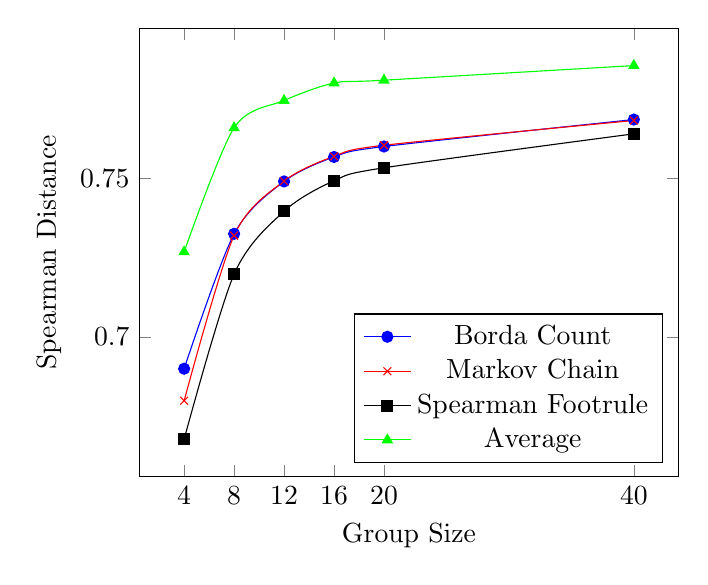
\begin{tikzpicture}
    \begin{axis}[
        xlabel=Group Size,
        ylabel=Spearman Distance,
        xtick = {4,8,12,16,20,40},
        legend pos=south east]
    \addplot[smooth,mark=*,blue] plot coordinates {
        (4,0.69)
        (8,0.7325)
        (12,0.749)
        (16,0.7567)
        (20,0.76)
        (40,0.7685)
    };
    \addlegendentry{Borda Count}

    \addplot[smooth,color=red,mark=x] plot coordinates {
            (4,0.6799)
            (8,0.73194)
            (12,0.7491)
            (16,0.7569)
            (20,0.7604)
            (40,0.7682)
        };
    \addlegendentry{Markov Chain}
    
        \addplot[smooth,color=black,mark=square*] plot coordinates {
            (4,0.6678)
            (8,0.7198)
            (12,0.7396)
            (16,0.7492)
            (20,0.7533)
            (40,0.764)
        };
    \addlegendentry{Spearman Footrule}
    
    \addplot[smooth,color=green,mark=triangle*] plot coordinates {
            (4,0.7268)
            (8,0.7659)
            (12,0.7745)
            (16,0.78)
            (20,0.7809)
            (40,0.7855)
        };
    \addlegendentry{Average}
    
    \end{axis}
\end{tikzpicture}
\caption{Results using SFD} \label{fig:footruledistance}
\end{figure}

\begin{table}[H]
	\centering
	\begin{tabular}{|l|lllll|}\hline
		& 4 to 8 & 8 to 12 & 12 to 16 & 16 to 20 & 20 to 40 \\ \hline
		BC 	& 6.16	& 2.25	& 1.03	& 0.44	& 1.12 \\
		MC  & 7.65	& 2.34	& 1.04	& 0.46	& 1.03 \\
		SF  & 7.79	& 2.75	& 1.30	& 0.55	& 1.42 \\
		Avg	& 5.38	& 1.12	& 0.71	& 0.12	& 0.59 \\ \hline
	\end{tabular}
	\caption{Percentage increase between the groups for SFD}
	\label{tbl:sfd}
\end{table}

Table \ref{tbl:sfd_ttest} shows the t-tests for SFD. BC and MC have two cases where the results are not distinct enough to be statistically different. BC and MC for group size 12 show the highest likelihood of of all comparisons to be indistinguishable.

\begin{table}[H]
	\centering
	\begin{tabular}{|l|llllll|}\hline
		& 4 & 8 & 12 & 16 & 20 & 40 \\\hline
		BC/MC	& $5e^{-86}$	& 0.027	& \textbf{0.875}	& \textbf{0.222}	& 0.0145 & 0.001 \\
		BC/SF	& $4e^{-265}$	& $3e^{-288}$	& $7e^{-295}$	& $2e^{-274}$	& $3e^{-277}$ & $2e^{-275}$ \\
		BC/Avg	& $7e^{-176}$	& $2e^{-254}$	& $5e^{-249}$	& $4e^{-253}$	& $5e^{-269}$ & $5e^{-297}$ \\
		MC/SF	& $7e^{-42}$	& $2e^{-243}$ 	& $1e^{-250}$	& $6e^{-258}$	& $2e^{-246}$ & $1e^{-242}$ \\
		MC/Avg	& $2e^{-217}$	& $2e^{-250}$ 	& $2e^{-248}$	& $2e^{-249}$	& $1e^{-265}$ & $1e^{-305}$ \\
		SF/Avg	& $2e^{-288}$	& 0	& 0	& 0	& 0 & 0 \\ \hline
	\end{tabular}
	\caption{P-values for SFD T-test}
	\label{tbl:sfd_ttest}
\end{table}